%----------------------------------------------------------------------------
\chapter{Wireframe-ek}
%----------------------------------------------------------------------------

A wireframe-ek egy alkalmazás tervezésénél nagyon gyakran elmaradnak, pedig igenis fontos szerepük van.
Rengeteg olyan dologra villágithatnak rá, amire egyébként nem gondolnánk és segíti a kommunikációt a fejlesztő(k) és a megrendelő között.

Ezeknek az elkészítéséhez a Figma névre keresztelt webes alkalmazást használtam. 
Ennek segítségével az egyszerű wireframe-ektől kezde komplex protoipizált design terveket is készíthetünk.


\begin{figure}[!ht]
  \centering
  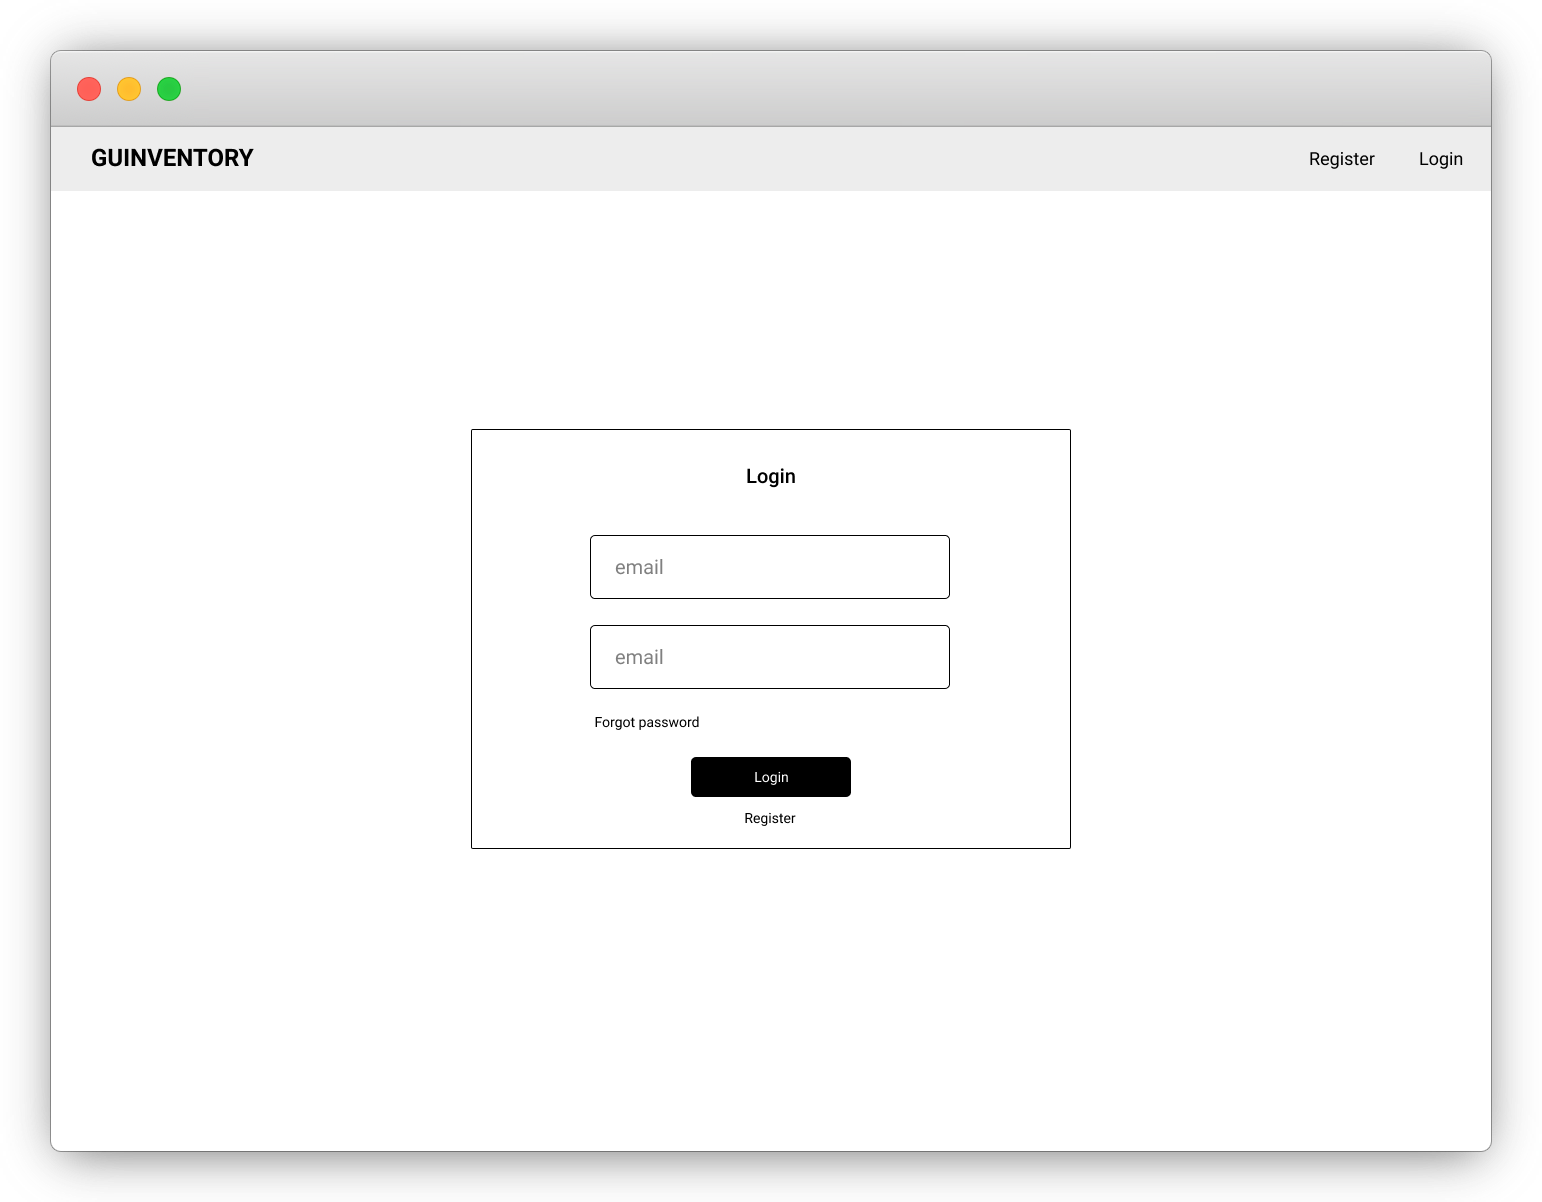
\includegraphics[width=150mm, keepaspectratio]{figures/wireframes/frame_login.png}
  \caption{Bejelentkezés wireframe}
  \label{fig:LoginWireframe}
\end{figure}

\begin{figure}[!ht]
  \centering
  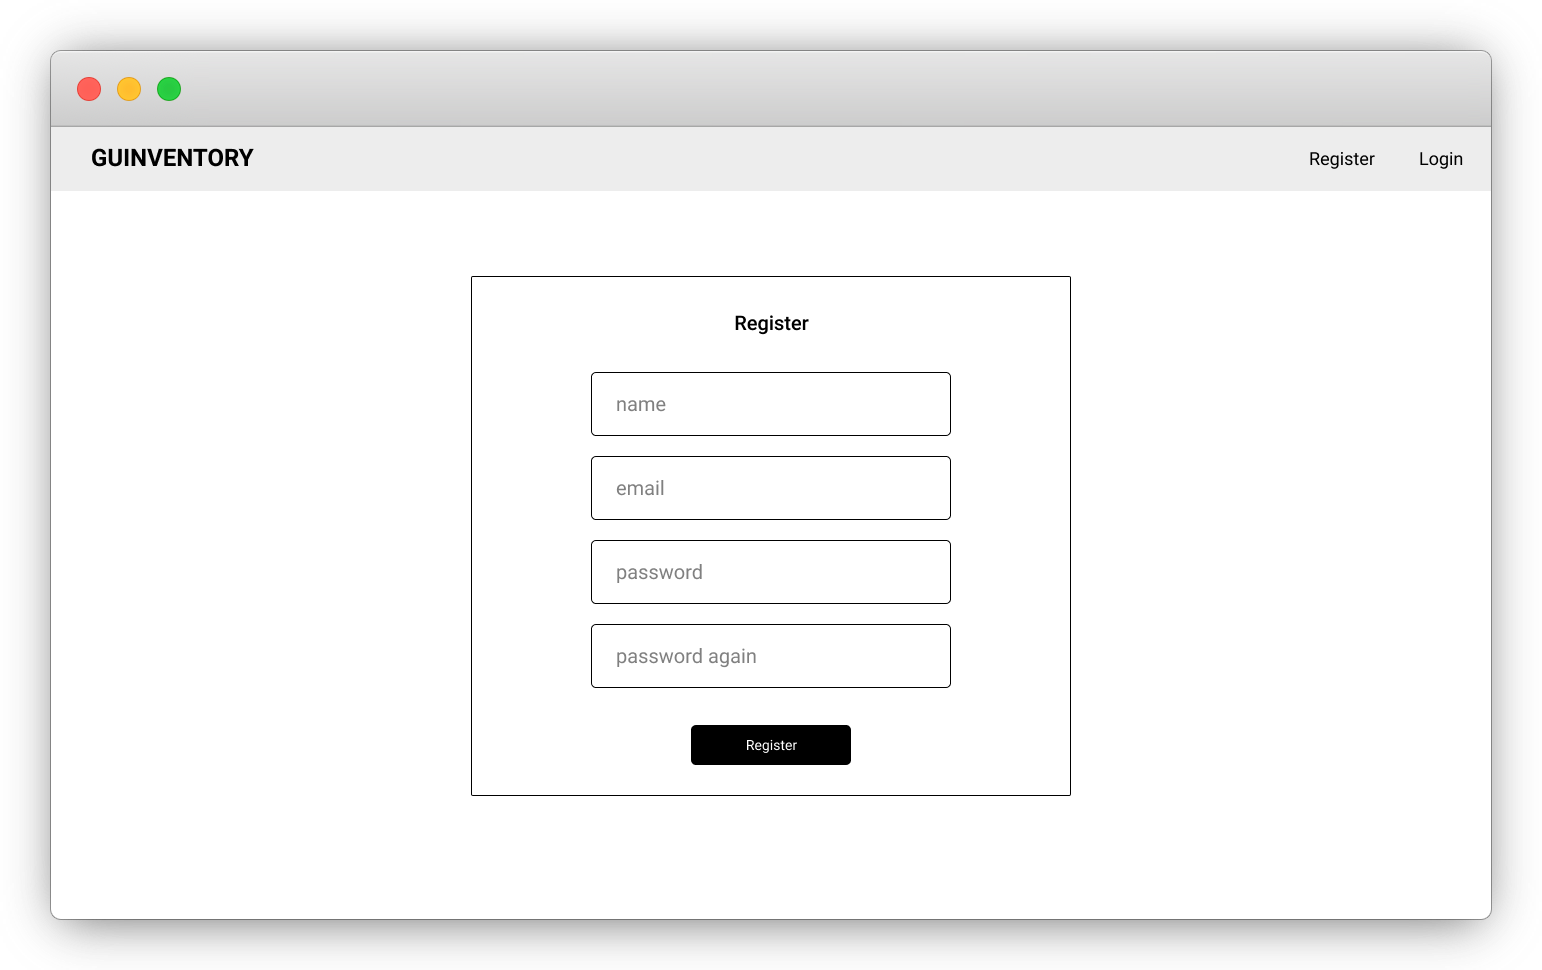
\includegraphics[width=150mm, keepaspectratio]{figures/wireframes/frame_registration.png}
  \caption{Regisztráció wireframe}
  \label{fig:RegistrationWireframe}
\end{figure}

\begin{figure}[!ht]
  \centering
  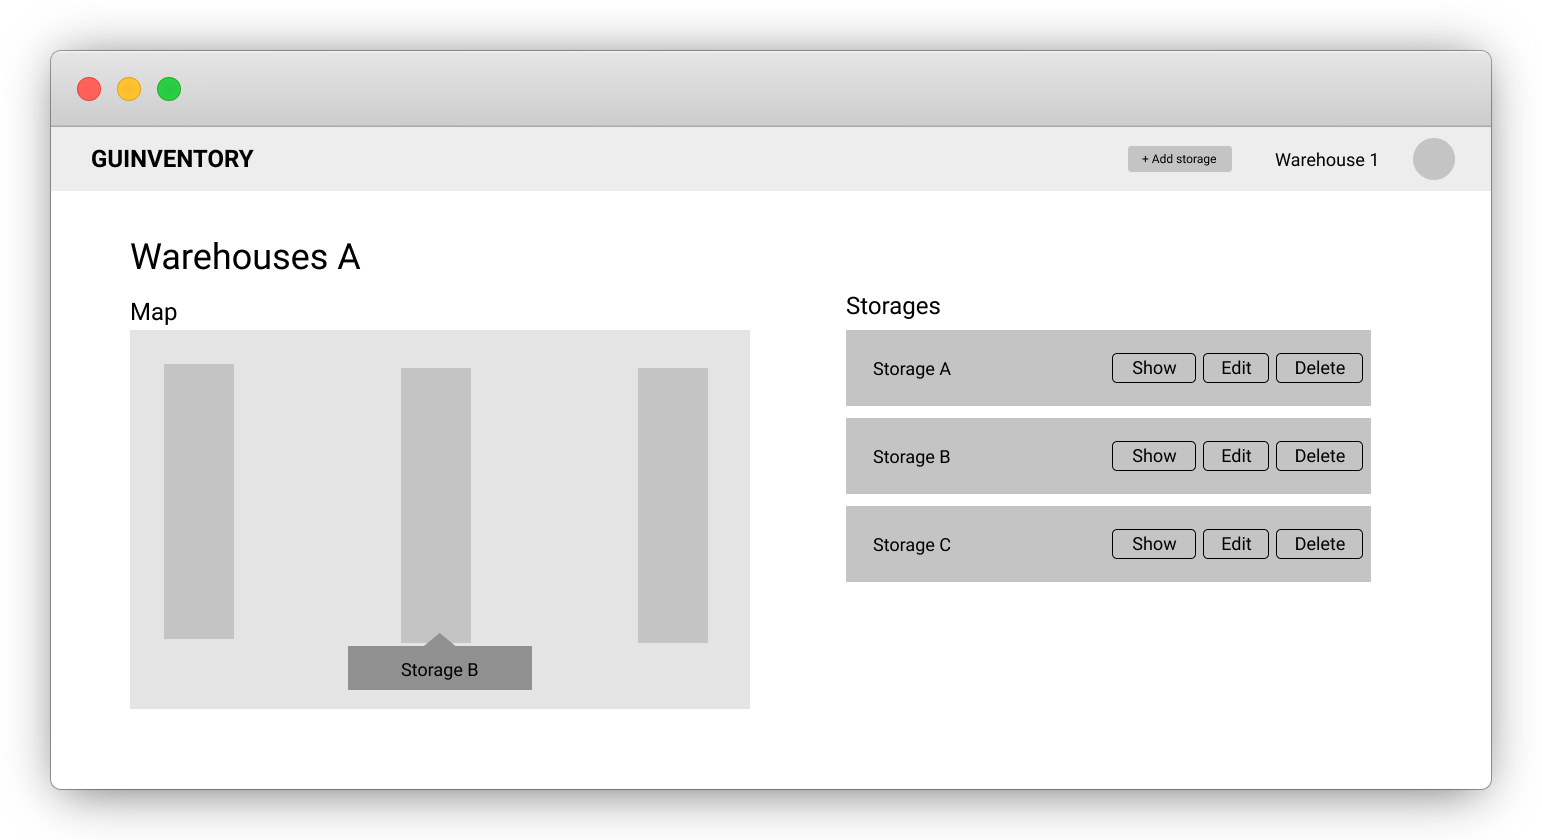
\includegraphics[width=150mm, keepaspectratio]{figures/wireframes/frame_warehouse.png}
  \caption{Raktár wireframe}
  \label{fig:WarehouseWireframe}
\end{figure}
  
\begin{figure}[!ht]
  \centering
  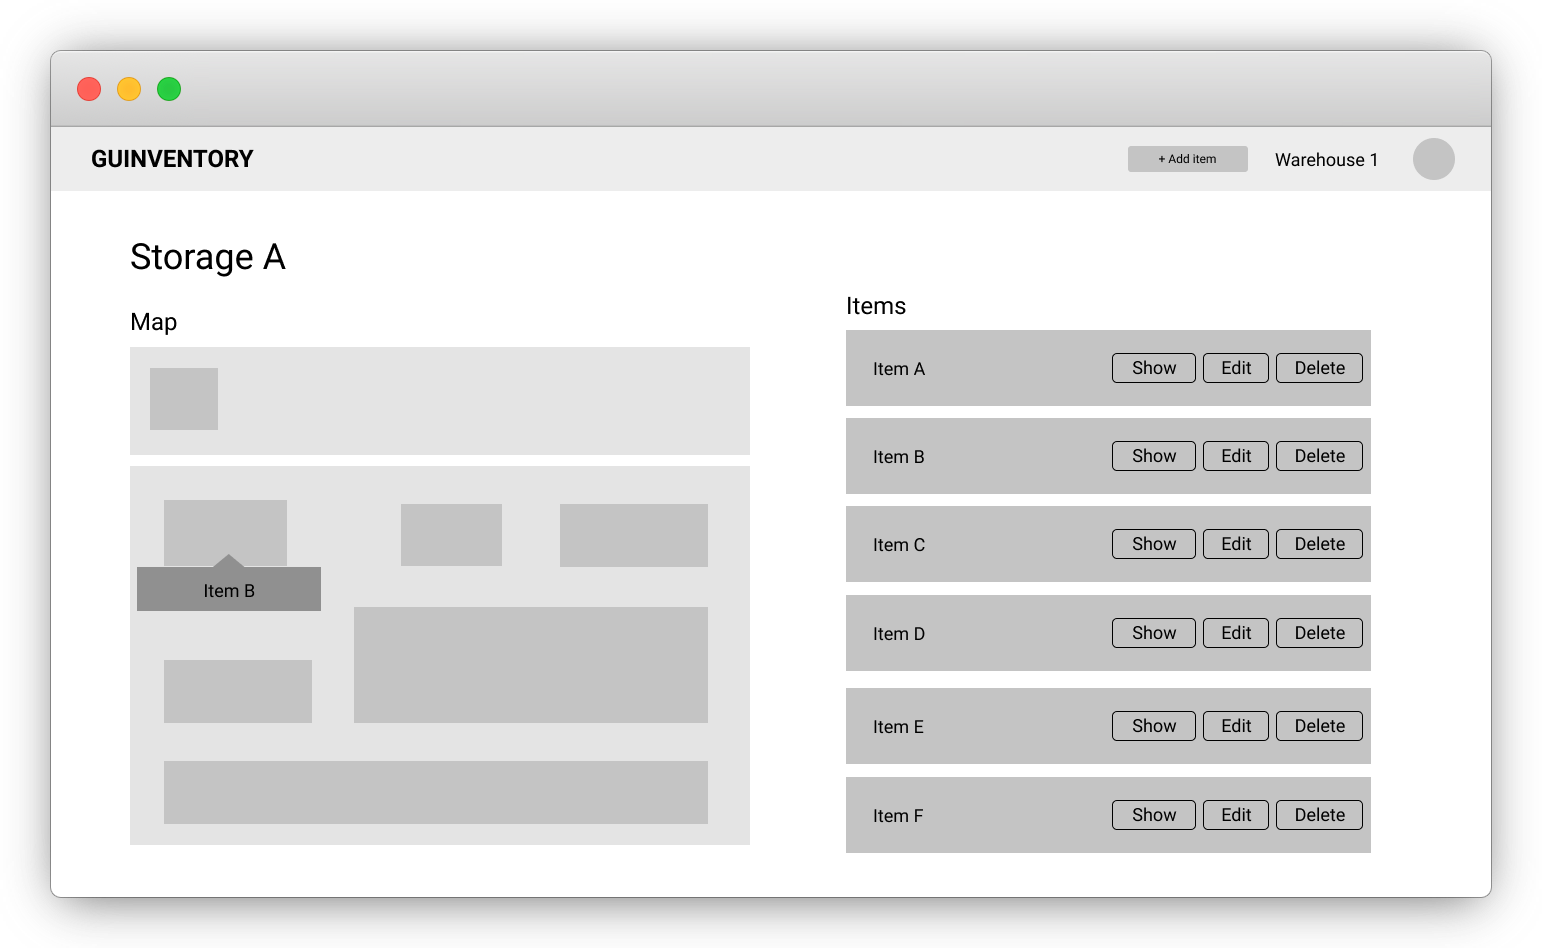
\includegraphics[width=150mm, keepaspectratio]{figures/wireframes/frame_storage.png}
  \caption{Tároló wireframe}
  \label{fig:StorageWireframe}
\end{figure}
  